% Chapter implemtation  

\chapter{Implementation} % Main chapter title

\label{implementation} % Change X to a consecutive number; for referencing this chapter elsewhere, use \ref{ChapterX}

\lhead{Chapter 5. \emph{Implementation}} % Change X to a consecutive number; this is for the header on each page - perhaps a shortened title

%----------------------------------------------------------------------------------------
%	SECTION 1
%----------------------------------------------------------------------------------------

%\colorbox{green}{Some introduction that motivates the work done in this thesis}

%\colorbox{green}{henvis til NS, nevn eksplisitt de ligningene som brukes}

%\colorbox{green}{Ta med et turbulensbilde, og bilde av plumen.}

This chapter aims to present the implementations done in this thesis. 
The routines implemented are meant to develop Nek5000 functionalities 
in the encounter with complex geometries. 

As shown in \fref{fig:mesh} the coarse element grid is created
in ICEM and then converted using the existing python script \verb|mshconvert| while the
distribution of GLL-nodes and the simulation itself was performed in Nek5000.
\verb|.rea| contains exact information about the corners,
limited information about the edges, and no information about the faces of the elements.
Hence the distribution of the GLL-nodes on a non-regular surface requires data exceeding the one in \verb|.rea|.
%For complex geometries and one part of this thesis has been to develop solutions that makes it 
%easier to work with complex geometries in Nek5000.

%The other part of the thesis has been to understand and apply Nek5000 with and without 
%LES to turbulent flow with gas dispersion and compare the results with reference 
%solutions from experiments and other solvers.

%The implementation is presented in 4 sections. The first two chapters describe two flow situations 
%used to compare Nek5000 with equivalent solvers and the two last chapters describe two distinct
%contributions to the mesh creating routine. 

\section{Project edges onto a specified arc} \label{xyzarc}

The Gordon Hall (GH) algorithm that is described in \cref{GH} was already implemented as a function in the Nek library.
By defining the GLL-nodes on the curved edges such that they correspond to an arc, the GH-algorithm is able to distribute 
the internal nodes accordingly. 

The curved edges are specified in \verb|.rea| and have until now been read as a second degree polynomial or as a part of a 
spherical shell. The routine \verb|xyzarc()| was created to process curved edges specified in \verb|.rea| with a radius and center.
It can be considered as an alternative to the already implemented \verb|xyzquad()| in \verb|genxyz.f| which generates curved edges 
represented as second order polynomials.
The algorithm is described below and \fref{fig:curvature} gives a visual representation of the situation.

The two end nodes of the edge are denoted $a$ and $b$. 
The mid node of the edge is named $c$, while 
%$s$ will be the arc length, 
$\theta$ is the full angle of the circle sector,
$cc$ is the center coordinates, 
$g$ denotes the vector containing the GLL-points in $[-1,1]$ 
and $r$ will be the radius.

\begingroup
%\fontsize{12pt}{14pt}
% s = r*|$\theta$|                       ! arc length
\begin{lstlisting}[escapechar=|,frame=none]
 l = a-b                       ! vector between the corner nodes
 c = (a+b)/2                   ! midpoint location
 h = c-cc                      ! height of the framed triangle
 |$\theta$| = arctan(abs(l)/2*abs(h))    ! half the angle of the circle sector
 g = g*|$\theta$|                      ! angles to the GLL-points on the circle-sector
 !---------- Finding the intersecting points ----------!
 !---- x on the line l, and extend x-cc to the arc ----!
 do k=1,lx1          ! for the number of nodes in one direction
    |$\alpha$| = h*tan(g[k])           ! offset from the midpoint on l
    x = c-|$\alpha$|*l/abs(l)           ! actual coordinate on l
    m = x-cc                   ! hypotenuse of the imposed triangle
    edge(k) = cc+r*m/abs(m)    ! final coordinate on the arc
 enddo
\end{lstlisting}
\endgroup
This code defines the GLL-nodes on a circle sector corresponding to the radius and circle center
provided in section \verb|CURVED SIDE DATA| in \verb|.rea|.
The remaining operation is to call the Gordon Hall algorithm and create the internal GLL-points.
%
\begin{figure}[h]
    \centering
    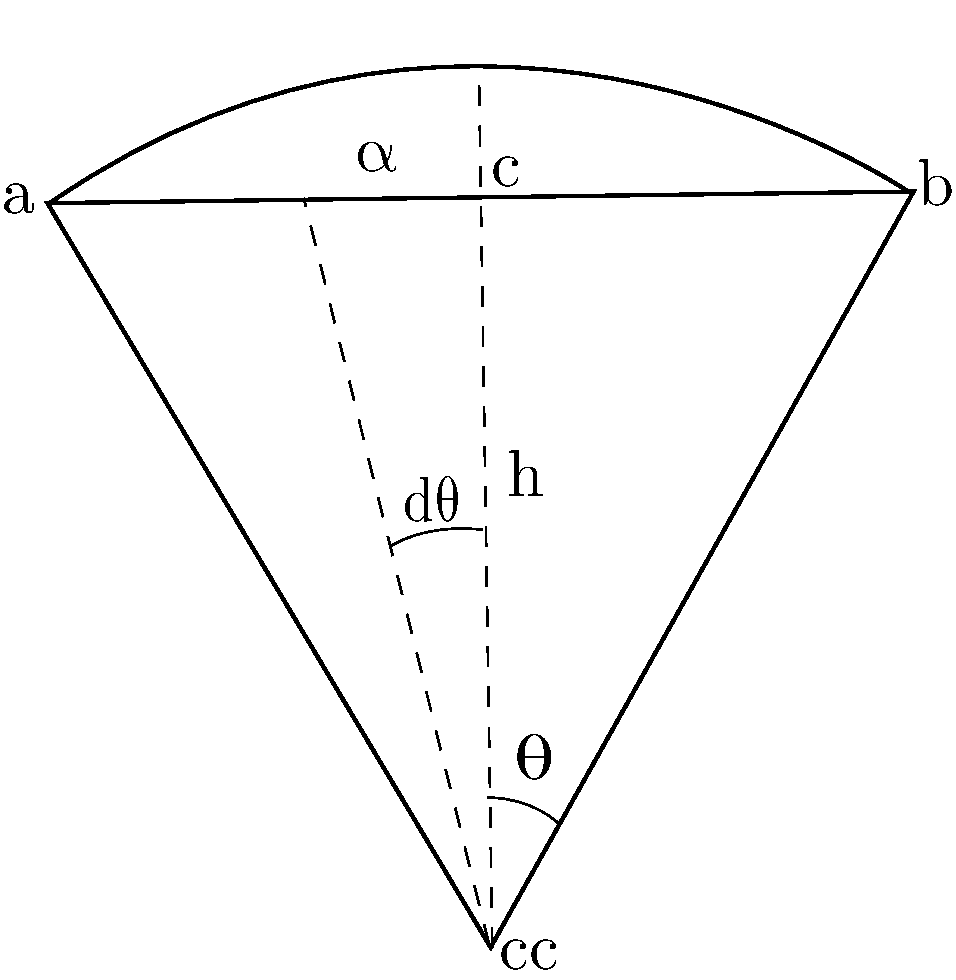
\includegraphics[width = 0.4\textwidth]{Figures/curvature.pdf}
    \caption{A sketch of the curved edge and the variables necessary to calculate the projection}
    \label{fig:curvature}
\end{figure}
%
To make this implementation fully automatic a small change in the script \verb|mshconvert| was also necessary. 
Since ICEM provides the midpoints of the curved edges, a function was added to convert the midpoint information 
originally provided to a circle center and its corresponding radius.
\section{General surface projection}\label{surfpro}
The routine \verb|xyzarc()| enables the user to more accurately represent circular edges.
For more complex geometry such as actual terrain and other surfaces without any analytic
expression the large element sizes make the geometrical representation difficult. 
Theoretically the GLL-points can be projected onto a non-analytical surface, but since 
the element mesh is created in a different program the necessary information is not available
to Nek5000. The idea is to create an additional fine surface mesh in ICEM such
that the nodes in this mesh describes the surface fine enough to distribute the GLL-nodes correctly in Nek5000.
During the initialization of the mesh in Nek5000 the program can read this information and project the GLL-nodes onto 
the provided surface. 
The routine was made as automatic as possible, and can be summarized in these three steps
\begin{enumerate}
    \item Create initial mesh and convert to \verb|.rea| applying \verb|mshconvert|.
        \item Create refined surface mesh on the non-regular surface.
        \item Enable projection by adding the line \verb|call surfprojection(n,a,b)|.
        %\item Choose number of interpolation points by modifying param(34)= (1,2,3)
\end{enumerate}

To explain the input parameters, let us first agree upon some naming conventions. 
The set of surface points is denoted $S$, while $f_e$ will denote the set of points 
in element $e$ that belong to the face that is going to be projected onto the surface described by $S$.
The number of interpolation points is denoted $n$, which has a maximum upper limit of three,
since the surface mesh is recommended to be a tetrahedra mesh. Setting $n=1$ simply projects 
a point in $f_e$ to the closest one in $S$.
The interpolation algorithm used for this experiment is an inverse distance interpolation
which applies the inverse distance squared as weights. The distance between a point
$\mathbf{x}\in f_e$, and a point $\mathbf{y} \in S $ is given as 
\begin{align}
    ||\mathbf{x}-\mathbf{y}||_{a} = a ||\mathbf{x}-\mathbf{y}||_{l^2}
    + (1-a)||\mathbf{n} - \frac{(\mathbf{x}-\mathbf{y})}{||\mathbf{x}-\mathbf{y}||_{l^2}}||_{l^2},
    \label{eq:distancenorm}
\end{align}
with $\mathbf{n}$ as the surface normal of the initial element face in the point $\mathbf{x}$.

The last parameter is provided to determine the size of the working array. 
The projection is done element wise, and to avoid unnecessary calculations a subset $S_e \subset S$
is used in~\eref{eq:distancenorm}.
Let $\mathbf{x}_e$ be the point at the center of face $f_e$
with radius $r_e$, the subset is then formulated as  
$S_e = \left\{ \mathbf{x} \in S , ||\mathbf{x}_e-\mathbf{x}|| < b \cdot r_e \right\}$.


In addition to the standard Nek5000 library the file \verb|surfpro.f| needs to be added to 
the folder \verb|trunk/nek/| along with all the other scripts applied by Nek5000.
This implementation could be done directly in \verb|.usr|, but it is of practical 
interest to keep this file as tidy as possible.
Two external files are also generated by the modified \verb|mshconvert| script for the algorithm to work.
\verb|surf.i| contains all the coordinates to the points on the refined surface. 
\verb|bdry.i| contains the element, and face number to all the faces to be projected onto the surface.

The algorithm is best explained through a simple box with a non-regular floor. 
An example of this situation is the hill of Ekeberg. 
Before describing the algorithm let $E_{tot} = n_xn_yn_z$  be the total number of elements, 
$N$ is the polynomial degree and let us for simplicity assume that $n_x=n_y=n_z$ such that 
$E= E_{tot}^{2/3}$ is the number of elements containing a face on the non-regular surface.
The number of points on the refined surface $N_s$ should be approximately $EN^4$ in 
order to describe the surface for all the GLL-points that belong to the boundary. This estimate
assumes that the surface mesh is equidistantly distributed whereas the GLL-nodes 
are denser along the boundaries of each element, $\Delta x_{min} = \mathcal{O}(1/N^2)$. 

The pseudo code for the algorithm is listed below with the temporal costs commented out.
%
\begingroup
\fontsize{12pt}{14pt}
\begin{lstlisting}[escapechar=|,frame=none]
do e,f in bdry.i   !O(E)
  wrk = create_working_surface(e,f)  !O(EN^4) 
  do i in GLL-nodes   !O(N^2)
    interp = init_interpolation_array() !O(1) 
    do j in wrk   !O(N^4)
       update_int_array(interp,wrk(j)) ! O(1)
    enddo
    set_new_point(interp,wrk,i,e,f) ! O(1)
  enddo
  fix_GLL() !O(N^3)
enddo
fix_geom()
\end{lstlisting}
\endgroup
% 
To understand the algorithm a short description of the auxiliary functions is 
given in the list below
\begin{itemize}
    \item create\_working\_surface(e,f) -- Loops through all the nodes in surf.i and adds the 
        surface-coordinates within a certain radius to the center of face $f$ on element $e$ to the array wrk.
        This saves time in the search for interpolation points for each GLL-node.
    \item init\_interpolation\_array() -- initializing the array containing the closest 
        points on the surface for the current GLL-node. 
    \item update\_int\_array(interp,wrk(j)) -- compares the current surface point to the 
        already existing interpolation points and adds it to the list if it is found to 
        be closer to the initial GLL-node.
    \item set\_new\_point(interp,wrk,i,e,f) -- updating the new GLL-point determined by the 
        surface points in interp.
    \item fix\_GLL() -- There is a risk after distributing the GLL-points on the surface that
        some of the internal GLL-points falls outside the element. This function distributes 
        all internal GLL-points correctly between the newly projected face and the opposite.
    \item fix\_geom() -- An already existing Nek routine that makes sure the manipulation of the 
        geometry is consistent with neighbouring elements, and distributes the internal GLL-points correctly.
\end{itemize}

Although this routine is only called once, and therefore will not contribute significantly 
to the total runtime of the program it is desirable to have a fast algorithm. Another analysis
important to be made is the amount of extra storage space needed for this algorithm.
By analysing the pseudo code the time of the algorithm should be of order $\mathcal{O}(E(EN^4+N^2N^4+N^3))=\mathcal{O}(EN^4(E+N^2))$
and the amount of additional storage space will be of order $\mathcal{O}(EN^4+E+N^2)=\mathcal{O}(EN^4)$.

The routine attempts to be as automatic as possible and the only implementation necessary is 
a call from \verb|usrdat2| with 3 input variables.

Now an illustrative example of how this method is applied by the user. Say you have a project
called ''myFlow'', and the mesh and surface mesh created in ICEM are named mesh\_myFlow and 
surfmesh\_myFlow. The following commands are then executed

%
%\begin{lstlisting}[style=FormattedNumber, basicstyle = \ttfamily,frame= none]
%>> ~/path/to/meshconvert/scrpt/nmshconvert --mesh mesh_myFlow 
%--reafile init.rea --outfile myFlow.rea
%--tol 1e3 --temperature True --curvetype A

%>> ~/path/to/meshconvert/scrpt/nmshconvert --mesh surfmesh_myFlow --mesh_format surface
%\end{lstlisting}
% 
\begingroup
\fontsize{12pt}{14pt}
\begin{lstlisting}[escapechar=|,frame=none]
>> /mshconvert --mesh mesh_myFlow 
    --reafile init.rea --outfile myFlow.rea
    --tol 1e-3 --temperature True --curvetype A

>> ./mshconvert --mesh surfmesh_myFlow 
    --mesh_format surface

\end{lstlisting}
\endgroup
After running the commands above the only thing left is to 
add \verb|call surfpro(n,a,b)| to \verb|usrdat2|.
% 
% 
%\begin{lstlisting}[style=FormattedNumber, frame=none]
    %int* p;
    %int a[4];
    %p = a;
%\end{lstlisting}
\subsection{Test of the projection routine}
To test the algorithm described in~\cref{surfpro} the hill of Ekeberg in Oslo 
and a helicopter body was used. These surfaces were loaded as \verb|.tin| files in ICEM and coarse hex meshes were created 
around the surfaces. The domains are presented in given in 
\fref{fig:surfpro}, notice the coarse element sizes in the figures.
These geometries were chosen because they resemble a typical problem with 
spectral elements. Since the initial element-mesh is relatively coarse it does not capture all 
the details in the geometry and the GLL-nodes distributed on the faces corresponding to the 
unstructured surface will be misplaced. 
%It is however no theoretical problem to reconstruct the surface with with a polynomial of order $P$. 
With the routine described in \cref{surfpro} the surface is approximated accurately 
by higher order polynomials.
%
\begin{figure}[h]
\centering
  \centerline{
\begin{minipage}{.5\textwidth}
  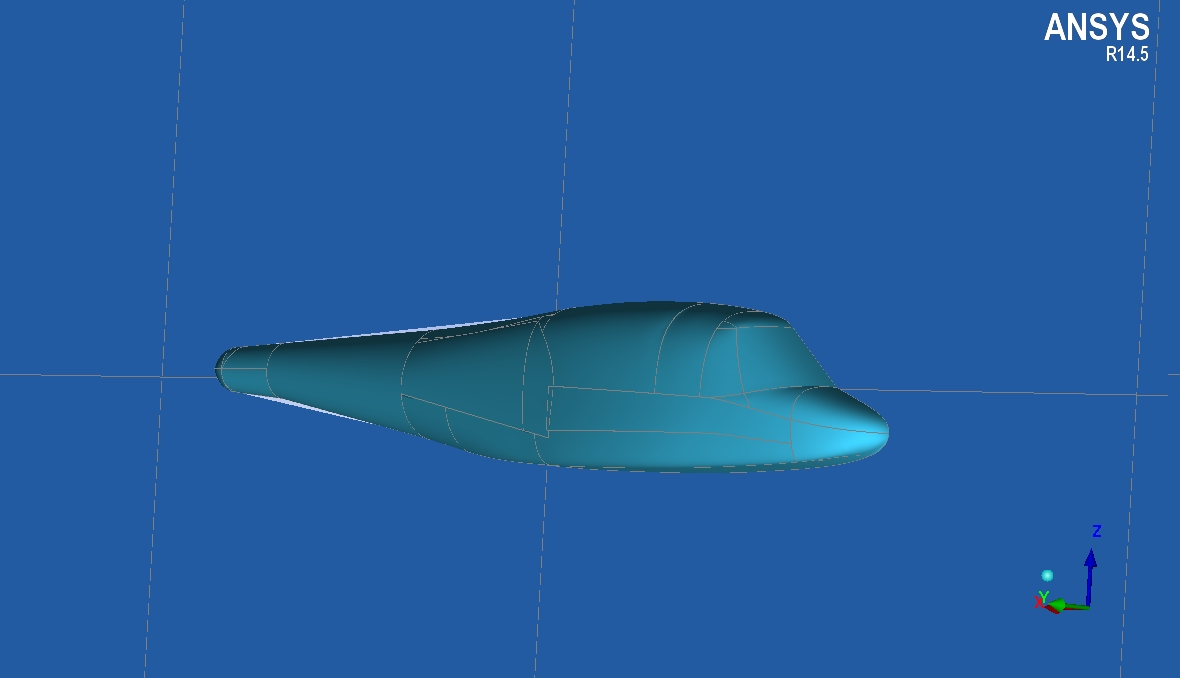
\includegraphics[width=1.0\linewidth]{Figures/helicopter.jpg}
  %\captionof{figure}{A figure}
\end{minipage}%
\begin{minipage}{.5\textwidth}
  \centering
  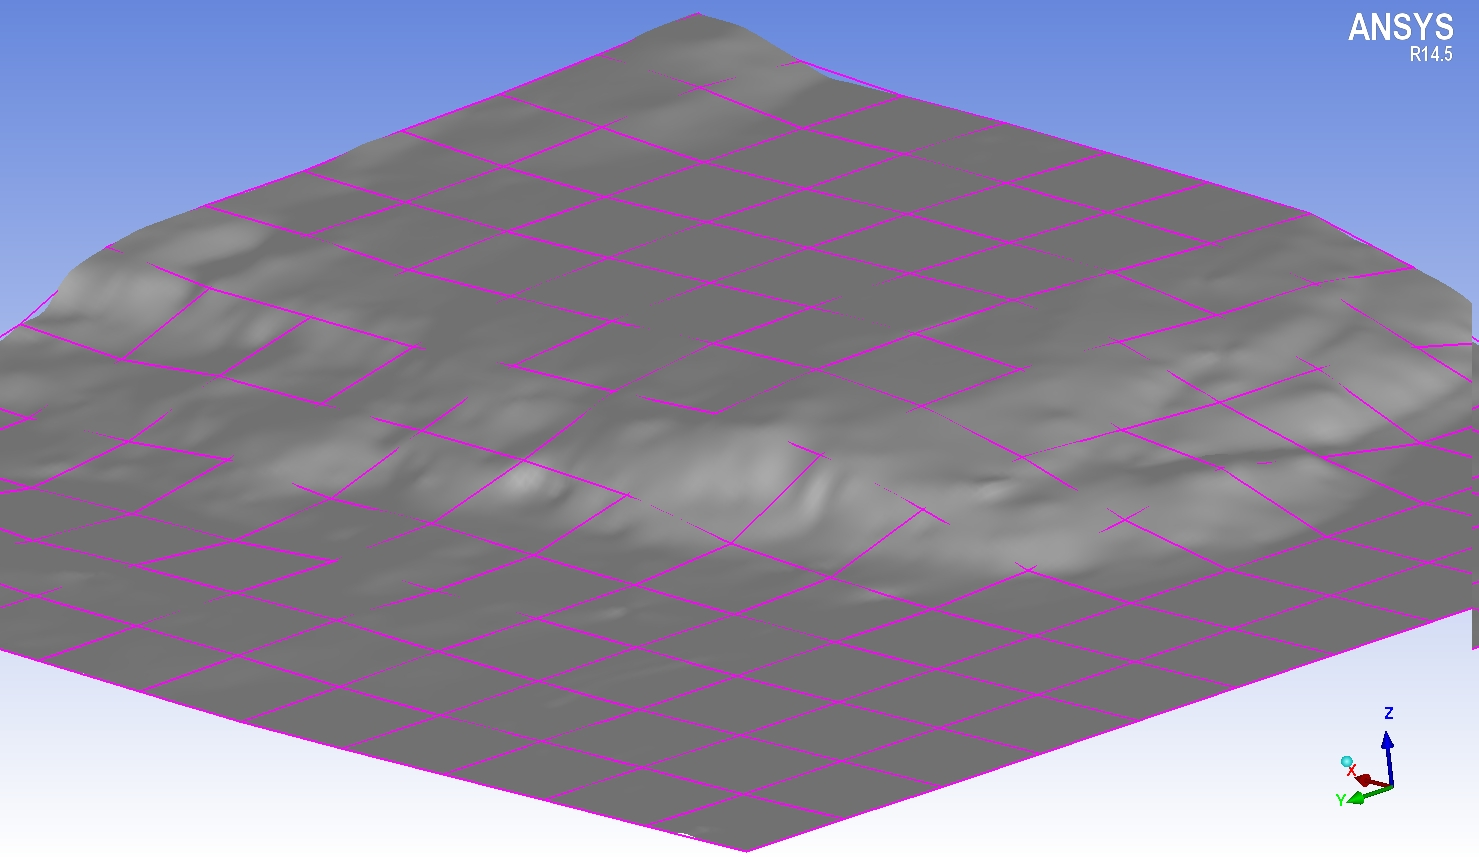
\includegraphics[width=1.0\linewidth]{Figures/mesh_ekeberg.jpg}
\end{minipage}
}
  \caption{Two examples of smooth surfaces with no analytical expression. 
  To the left is the body of a helicopter, to the right is the hill of Ekeberg.}
  \label{fig:surfpro}
\end{figure}
%
The algorithm restricts itself to relatively smooth surfaces, since the polynomial 
describing the surface is typically of order $P \approx 7$.
%
\section{Spatial averaging routine}
A dynamic Smagorinsky model has previously been implemented in Nek5000 for flow in a channel. 
The SGS-model as described in \cref{description} depends on an averaging routine to calculate
the dynamic Smagorinsky constant. The previous implementation in Nek5000 applies a planar average routine
in addition to averaging in time. The planar averaging is based on the assumption that the Smagorinsky 
constant is the same for all points with equal distance to the walls of the channel.
This is a case specific averaging routine based on the assumption of homogeneous turbulence 
in the entire plane, hence only applicable to flows in idealized geometries.

When applying dynamical Smagorinsky to Case 1 a new spatial mean routine had to be applied for it to be stable. 
It was first attempted to average only in time, but this proved not to be sufficient. It was
therefore implemented a routine for taking the average within each element, let 
$c_{num}^e,c_{den}^e$ denote the numerator and the denominator in \eref{eq:dynsmag}.
The means are then calculated as 
\begin{align}
    c_{num}^e = \frac{1}{V}\int_{\Omega_e}c_{num}^e d\: \Omega 
    \approx \frac{1}{V}\sum_{i = 1}^{N^3}\rho_{i,e}c_{num,i}^{e}.
    \label{eq:averageroutine}
\end{align}
And similarly for $c_{den}^e$.
The coefficients $\rho_{i,e}$ are found in the array \verb|BM1(lx1,ly1,lz1)| in the file 
\verb|MASS|.
